\documentclass[11pt,a4paper,twoside,openright,bibliography=totoc]{scrbook}

\usepackage{graphicx,xcolor}
\usepackage{amssymb,amsmath,array}

% Color citation, references and links.
\usepackage[]{hyperref}
\hypersetup{
  colorlinks,
  linkcolor={black},
  citecolor={red!70!black},
  urlcolor={blue!70!black}
}

\begin{document}
% Example of title page for the projects carried out within the lasec 

% Simply include it in your mastex tex file: 
%        % Example of title page for the projects carried out within the lasec 

% Simply include it in your mastex tex file: 
%        % Example of title page for the projects carried out within the lasec 

% Simply include it in your mastex tex file: 
%        \input{cover}


% Updated March 2006 (SP)


\newcommand{\logoepfl}[0]{
  \begin{center}
    \includegraphics[width=4cm]{cover/logo_epfl_coul.eps}
  \end{center}
  \vspace{0.3cm}
  \hrule
}
\newcommand{\logolasec}[0]{
  \vspace{1cm}
  \hrule
  \begin{center}
    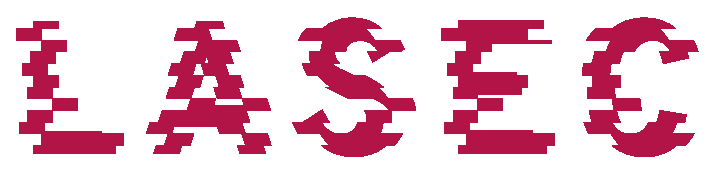
\includegraphics[width=4.5cm]{cover/logo_lasec_coul.eps}
  \end{center}
}
\newcommand{\project}[1]{
  \begin{center}
    \large{#1}
  \end{center}
  \vspace{1cm}
}
\newcommand{\department}[1]{
  \begin{center}
    \large{#1}
  \end{center}
}
\newcommand{\supervisor}[3]{
  \begin{center}
    \begin{normalsize}{
        \bfseries #1}\\#2\\#3
    \end{normalsize}
  \end{center}
}
\renewcommand{\author}[1]{
  \begin{center}
    \Large{#1}
  \end{center}
  \vspace{0.5cm}
}
\renewcommand{\title}[1]{
  \vspace{3cm}
  \begin{center}
    \huge{#1}
  \end{center}
  \vspace{1.7cm}
}
\renewcommand{\date}[2]{
  \begin{center}
    \normalsize{#1 #2}
  \end{center}
  \vspace{0.5cm}
}


\thispagestyle{empty}


% begin title page
\logoepfl

\title{Messaging Application with Ratcheting Security}

\author{Andrea Caforio}
\department{School of Computer and Communication Sciences}
\project{Optional Semester Project}

\date{January}{2019}

\begin{center}
  \begin{tabular}{cc}
    \begin{tabular}{p{4.0cm}}
      \supervisor{Responsible}{Prof. Serge Vaudenay}{EPFL / LASEC}
    \end{tabular}&
    \begin{tabular}{p{4.0cm}}
      \supervisor{Supervisor}{Dr. Betül Durak}{EPFL / LASEC}
    \end{tabular}
  \end{tabular}
\end{center}

\logolasec
% end title page




% Updated March 2006 (SP)


\newcommand{\logoepfl}[0]{
  \begin{center}
    \includegraphics[width=4cm]{cover/logo_epfl_coul.eps}
  \end{center}
  \vspace{0.3cm}
  \hrule
}
\newcommand{\logolasec}[0]{
  \vspace{1cm}
  \hrule
  \begin{center}
    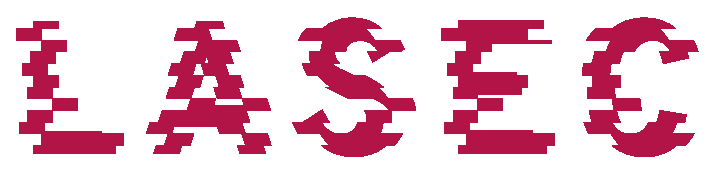
\includegraphics[width=4.5cm]{cover/logo_lasec_coul.eps}
  \end{center}
}
\newcommand{\project}[1]{
  \begin{center}
    \large{#1}
  \end{center}
  \vspace{1cm}
}
\newcommand{\department}[1]{
  \begin{center}
    \large{#1}
  \end{center}
}
\newcommand{\supervisor}[3]{
  \begin{center}
    \begin{normalsize}{
        \bfseries #1}\\#2\\#3
    \end{normalsize}
  \end{center}
}
\renewcommand{\author}[1]{
  \begin{center}
    \Large{#1}
  \end{center}
  \vspace{0.5cm}
}
\renewcommand{\title}[1]{
  \vspace{3cm}
  \begin{center}
    \huge{#1}
  \end{center}
  \vspace{1.7cm}
}
\renewcommand{\date}[2]{
  \begin{center}
    \normalsize{#1 #2}
  \end{center}
  \vspace{0.5cm}
}


\thispagestyle{empty}


% begin title page
\logoepfl

\title{Messaging Application with Ratcheting Security}

\author{Andrea Caforio}
\department{School of Computer and Communication Sciences}
\project{Optional Semester Project}

\date{January}{2019}

\begin{center}
  \begin{tabular}{cc}
    \begin{tabular}{p{4.0cm}}
      \supervisor{Responsible}{Prof. Serge Vaudenay}{EPFL / LASEC}
    \end{tabular}&
    \begin{tabular}{p{4.0cm}}
      \supervisor{Supervisor}{Dr. Betül Durak}{EPFL / LASEC}
    \end{tabular}
  \end{tabular}
\end{center}

\logolasec
% end title page




% Updated March 2006 (SP)


\newcommand{\logoepfl}[0]{
  \begin{center}
    \includegraphics[width=4cm]{cover/logo_epfl_coul.eps}
  \end{center}
  \vspace{0.3cm}
  \hrule
}
\newcommand{\logolasec}[0]{
  \vspace{1cm}
  \hrule
  \begin{center}
    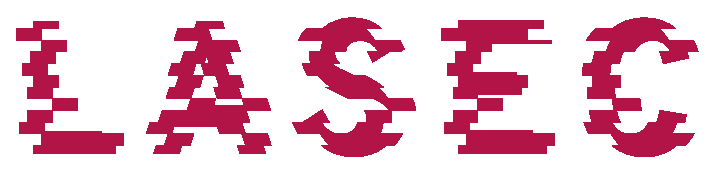
\includegraphics[width=4.5cm]{cover/logo_lasec_coul.eps}
  \end{center}
}
\newcommand{\project}[1]{
  \begin{center}
    \large{#1}
  \end{center}
  \vspace{1cm}
}
\newcommand{\department}[1]{
  \begin{center}
    \large{#1}
  \end{center}
}
\newcommand{\supervisor}[3]{
  \begin{center}
    \begin{normalsize}{
        \bfseries #1}\\#2\\#3
    \end{normalsize}
  \end{center}
}
\renewcommand{\author}[1]{
  \begin{center}
    \Large{#1}
  \end{center}
  \vspace{0.5cm}
}
\renewcommand{\title}[1]{
  \vspace{3cm}
  \begin{center}
    \huge{#1}
  \end{center}
  \vspace{1.7cm}
}
\renewcommand{\date}[2]{
  \begin{center}
    \normalsize{#1 #2}
  \end{center}
  \vspace{0.5cm}
}


\thispagestyle{empty}


% begin title page
\logoepfl

\title{Messaging Application with Ratcheting Security}

\author{Andrea Caforio}
\department{School of Computer and Communication Sciences}
\project{Optional Semester Project}

\date{January}{2019}

\begin{center}
  \begin{tabular}{cc}
    \begin{tabular}{p{4.0cm}}
      \supervisor{Responsible}{Prof. Serge Vaudenay}{EPFL / LASEC}
    \end{tabular}&
    \begin{tabular}{p{4.0cm}}
      \supervisor{Supervisor}{Dr. Betül Durak}{EPFL / LASEC}
    \end{tabular}
  \end{tabular}
\end{center}

\logolasec
% end title page


\tableofcontents

\chapter{Introduction}
\label{chap:introduction}

Messaging has become an ubiquitous resource in the daily lives of
millions of people around the globe through the widespread adoption of
instant messaging applications. The design of protocols which
facilitate securing messaging or key-agreement is faced with a unique
set of challenges, this is due to the longevity of sessions between
communicating parties and the inherently asynchronous notion of
messaging where a participant is both the sender and recipient of
messages and the time a message is sent or received is undefined. In
such a setting the leakage of a state to the adversary is especially
devastating since in a naive protocol it would not only enable him to
recover past messages but also allow future impersonations of the
victim. Ratcheting has established itself as the go-to technique in
order to mitigate these risks. Akin to its mechanical equivalent the
states are continuously moved forward (updated) without the
possibility of going backwards, i.e.~it should be impossible to
recover past states from the current one. This further implies that
past message remain secure even in the presence of and adversary who
can expose the state of a participant. The literature labels protocols
that deploy ratchets as \textit{forward-secure}. This technique saw
its inception in 2004 as part of the Off-the-Record messaging
protocol~\cite{borisov2004off}. It only recently gained traction
through the massively popular Signal protocol. The release of this
protocol however predates its first formal security analysis in 2017
and since then several novel protocols with various degrees of
security levels have been proposed~\cite{cohn2017formal}. Among others
these protocols also attempt the satisfy the notion of \textit{future
secrecy} in which future states and messages remain secure even if the
current state has been leaked. Furthermore, a secure messaging
protocol should be efficient enough to run smoothly even on
computationally inferior devices thus the choice of fast primitives
that do not compromise the promised security levels play a crucial
part in the construction of messaging protocols. Even though on paper
the attained levels of security in these new protocol often only
differ marginally the effects on performance metrics are of a
different kind with sometimes huge differences between the protocols.

% Add some more text here.

\section{Contributions}
\label{sec:contributions}

This project is concerned with surveying and solidifying the
performance differences of six new secure messaging or key-update
protocols that have been proposed during the past two years. In
chapter~\ref{chap:protocols} the notion of secure messaging and
especially ratcheting is formally reviewed before each protocol is
summarized in terms of composition and security levels, then in
chapter~\ref{chap:benchmarks} the protocols are measured and compared
on the basis of several benchmarks. In chapter~\ref{chap:bark} we
extend and modify the in-house Bidirectional Asynchronous Ratcheted
Key Agreement protocol (BARK) proposed by the LASEC laboratory into a
faster version with only minor concessions in terms of security before
concluding this report in the last chapter.

\section{Circumstances}
\label{sec:circumstances}

This project has been conducted as part of the third master semester optional
semester project in computer science course (CS-596) offered by the
School of Computer and Communications Sciences at EPFL and is credited
with eight points. It was supervised by Doctor Betül Durak of
the LASEC laboratory.

\chapter{Protocols}
\label{chap:protocols}

\chapter{Benchmarks}
\label{chap:benchmarks}

\chapter{On-Demand BARK}
\label{chap:bark}

\chapter{Conclusion}
\label{chap:conclusion}


\bibliographystyle{plain}
\bibliography{bibliography}

\end{document}
